\section{Canal Parabólico}
\label{sec:canal}

\begin{problem}
  Realice una el trazados de rayos de un canal parabólico que tiene un ángulo de borde $\psi = 80^\circ$, y un ancho de apertura de 1.5~m.
\end{problem}

\TheSolution Sabemos que de la ecuación~\ref{eq:rhof} podemos calcular el foco $f$ de la parabóla, dado que conocemos el ángulo de borde $\psi = 80^\circ$ y sabemos que $x_b = \rho \sin \psi_b$ en donde $x_b= 0.75$, debido a que la apertura es de 1.5~m. Calculamos $\rho$ que es igual a 0.76~m. Considerese la Figura~\ref{fig:canal}.

\begin{figure}[ht]
  \centering
  \includegraphics[width=1.0\textwidth]{figures/canalP}
  \caption{\label{fig:canal} Parabóla del concentrador de canal parabólico.}
\end{figure}

\begin{equation}
  \label{eq:rhof}
  \rho = \dfrac{2 f}{1 + \cos \psi_b}
\end{equation}
despejando $f$ y sustituyendo los valores correspondientes $f = 0.4469$~m.

Por otro lado, sabemos que el área de apertura es $A_p = (2 x_b) L$, por lo que podemos considerar una $L= 3$~m. Para el calculo del receptor utilizamos la ecuación~\ref{eq:diametro2}, nuevamente, en donde consideraremes el semi-ángulo de aceptación $\Delta = 4.65\rm mrad$ igual al tamaño del cono solar.

\begin{equation}
  \label{eq:diametro2}
  D = \dfrac{4 \Delta_r f}{1 + \cos \psi_b}
\end{equation}
sustituyendo los valores podemos calcular que el díametro ideal del receptor que es igual a 7.08~mm.

\ASolution Para la simulación de trazado de rayos utilizamos utilizamos un vector solar $\hat s = (0,0,1)$, una función \emph{Pillbox} forma solar. Las propiedades ópticas del concentrador se muestran en la Tabla~\ref{tab:opticaCanal}


\begin{table}[h]
  \centering
  \begin{tabular}[h]{ccccc}
    \toprule
    Reflectivity & Transmissivity & Slope error & Specularity error & Error type\\
    \midrule
    0.96         & 0.0001         & 0.0001      & 0.0001            & Gaussian\\
    \bottomrule
  \end{tabular}
  \caption{\label{tab:opticaCanal} Propiedades ópticas}
\end{table}

Se generan dos etapas una para el concentrador y otra para el receptor. Para simular un canal parabólico se selecciona la apertura \emph{Rectangular} y se considera una longitud de 3~m. Se utiliza una superficie parabólica con el foco calculado. La interacción es de reflexión y los parámetros ópticos los definidos con anterioridad.

\begin{table}[h]
  \centering
  \scriptsize
  \begin{tabular}[h]{lllllllll}
    \toprule
    X-C & Y-C & Z-C & X-AimP & Y-AimP & Z-AimP & Z-Rot & Aperture & Surface\\
    \midrule
    0 & 0 & 0 & 0 & 0 & 1 & 0 & r--0.75,3,0,0,0,0,0,0 & p-1.1213,0,0,0,0,0,0,0\\
    \bottomrule
  \end{tabular}
  \caption{\label{tab:etapaReceptorD} Etapa del concentrador.}
\end{table}

Las propiedades del receptor se muestran en la Tabla~\ref{tab:etapaRecC}, donde el receptor lo colocamos en el foco. La apertura también es del tipo \emph{Single Axis Curvature Section} con una longitud de 3~m. La superficie es de tipo cilindrico con el díamero calculado.
\begin{table}[h]
  \centering
  \scriptsize
  \begin{tabular}[h]{lllllllll}
    \toprule
    X-C & Y-C & Z-C & X-AimP & Y-AimP & Z-AimP & Z-Rot & Aperture & Surface\\
    \midrule
    0 & 0 & 0.4469 & 0 & 0 & -1 & 0 & l-0,0,3,0,0,0,0,0 & t-282.486,0,0,0,0,0,0,0\\
    \bottomrule
  \end{tabular}
  \caption{\label{tab:etapaRecC} Etapa del receptor }
\end{table}

Realizando un simulación para con un millón de rayos se obtienen los resultados mostrados en la Figura~\ref{fig:canal}.

\begin{figure}[ht]
  \centering
  \subfigure[]{
    \includegraphics[width=0.41\textwidth]{figures/canal}}
  \subfigure[]{
    \includegraphics[width=0.48\textwidth]{figures/fluxCanal}}
  \caption{\label{fig:canal} Trazado de rayos del un canal parabólico.}
\end{figure}

%%% Local Variables: ***
%%% mode: latex ***
%%% TeX-master: "taller.tex" ***
%%% End: ***
